\documentclass{standalone}
\usepackage[utf8]{inputenc}
\renewcommand*\familydefault\sfdefault

\title{CIS 114 Final Project Proposal - UML Use Case Diagram}
\author{Leomar Durán}
\date{27 November 2021}

%%%%%%%%%%%%%%%%%%%%%%%%%%%%%%%%%%%%%%%%%%%%%%%%%%%%%%%%%%%%%%%
% CHANGELOG :
%     2021-12-06t22:39
%         implemented `\findarrlen` to find length of arrays
%
%     2021-11-27t15:37
%         integrated all actor loops
%
%     2021-11-27t15:37
%         loop to place actors
%         better loop variables in \actor
%
%     2021-11-27t15:13
%         actor labels, associations in loop,
%         better loop variables in document
%
%     2021-11-27t03:45
%         detailed administrator, looped repetitive tasks
%
%     2021-11-27t03:15
%         associated user to their use cases
%
%     2021-11-27t03:08
%         add the user and first server actor
%
%     2021-11-27t01:24
%         create the package of use cases
%
%     2021-11-26t20:37
%         documented \actor[5][1]
%
%     2021-11-26t20:25
%         added ports to actor
%
%     2021-11-26t16:40
%         created actor shapes
%
%     2021-11-26t14:53
%         started with an empty node
%%%%%%%%%%%%%%%%%%%%%%%%%%%%%%%%%%%%%%%%%%%%%%%%%%%%%%%%%%%%%%%

\usepackage{tikz} % for tikzpicture
\usetikzlibrary{calc}
\usetikzlibrary{positioning}
\usetikzlibrary{intersections}
\usetikzlibrary{matrix}
\usetikzlibrary{shapes}

% The actor shape without scope or ports
\newcommand*\unscopedactor{%
    \draw (0,22.5pt) circle (7.5pt);% head
    \draw (0,15pt) -- ++(0,-25pt) -- ++(-15pt,-20pt);% body and left leg
    \draw (-15pt,10pt) -- ++(30pt,0);% arms
    \draw (0,-10pt) -- ++(15pt,-20pt)% right leg
}%

% The actor shape including scope and ports
% @param * adds the last x/y-coordinates to x/y-shifts
% @param 1 scale (default 1)
% @param 2 port name prefix
% @param 3 x-shift
% @param 4 y-shift
% @param 5 extensions after the actor within scope
\makeatletter
    \newcommand*\actor{%
        \@ifstar%
            \actor@star%
            \actor@nostar%
    }%
    \newcommand*\actor@star[5][1]{%
        % coordinates stored for positioning actors
        \newdimen\xcoord
        \newdimen\ycoord
        \pgfgetlastxy\xcoord\ycoord;%
        \actor@nostar[#1]{#2}{\xcoord+#3}{\ycoord+#4}{#5}%
    }%
    \newcommand*\actor@nostar[5][1]{%
        \begin{scope}[scale=#1,xshift=#3,yshift=#4,line width=1pt]%
            \unscopedactor;%
            % create the actor ports
            % \port actor port
            % \x/\y actor coordinates
            \foreach \port/\x/\y in {%
                /0/0,% central port
                -north/0/30pt,%
                -west/-15pt/10pt,%
                -east/15pt/10pt,%
                -south/0/-30pt%
            }{%
                \coordinate (#2\port) at (\x,\y);%
            } % \foreach \port/\x/\y
            #5%
        \end{scope}%
    }%
\makeatother%

% Finds the number of elements in the array given by #1.
% @param 1 array to iterate
% @param 2 counter name
\newcommand*\findarrlen[2]{%
    \setcounter{#2}0%
    \foreach\tmp in #1{%
        \stepcounter{#2}%
    }%
}%

% echos directions
\def\echoeast{east}
\def\echowest{west}

\begin{document}

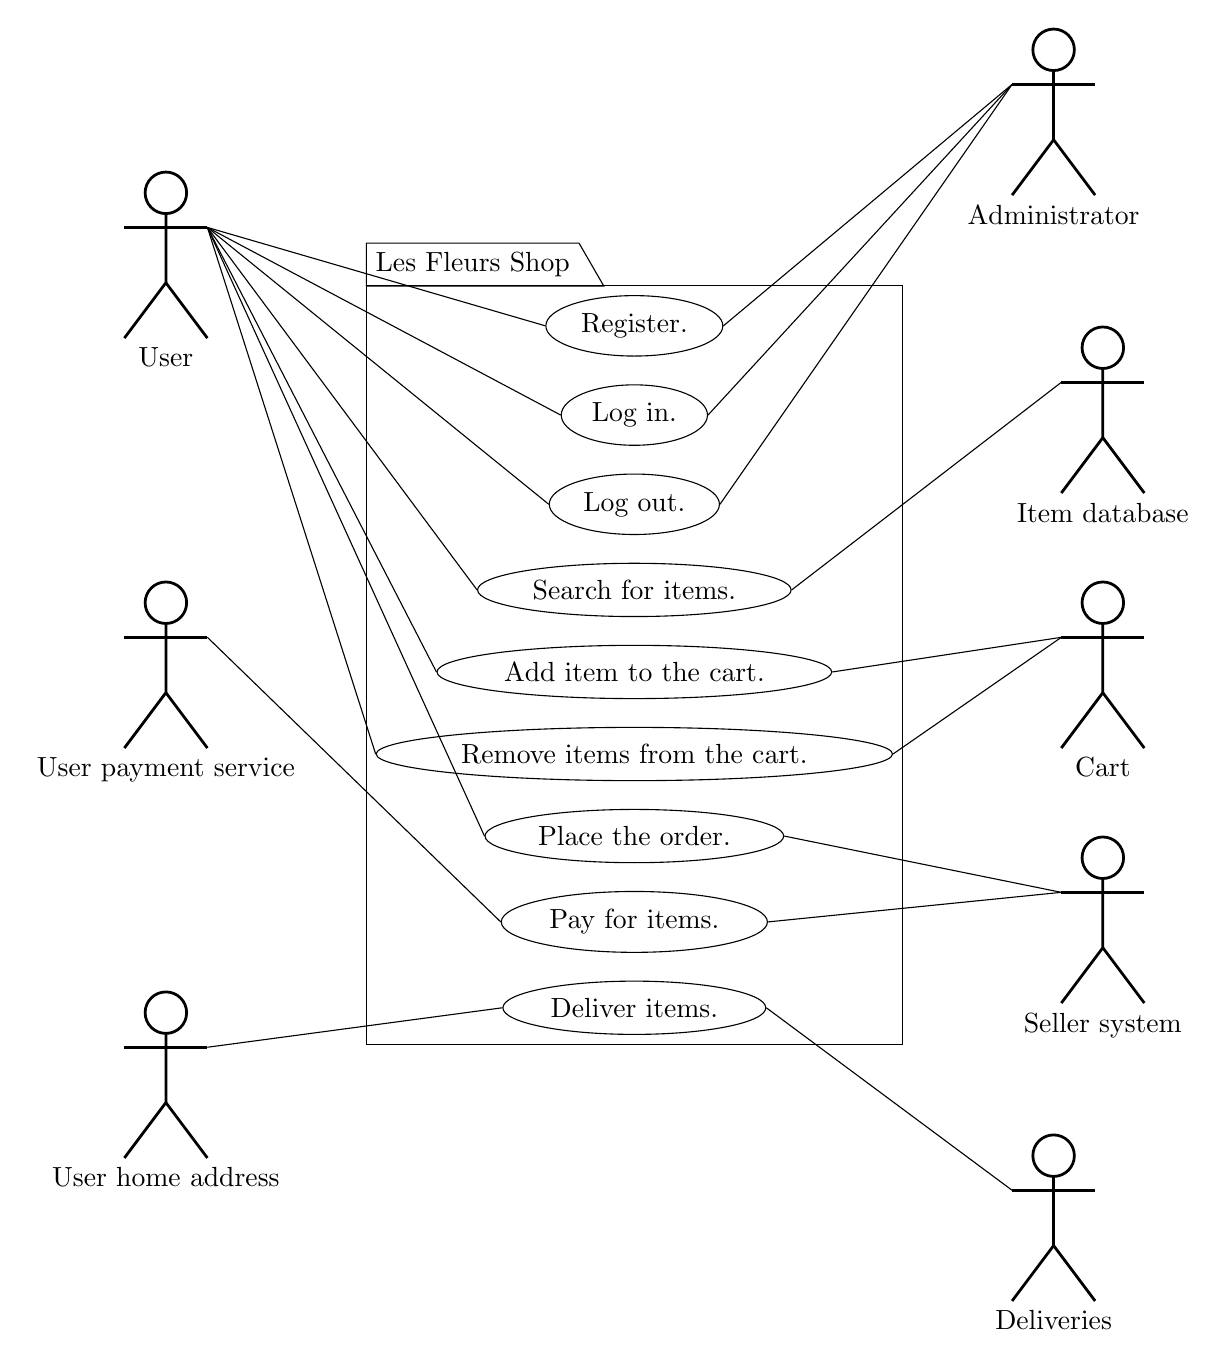
\begin{tikzpicture}
    [%
        package head/.style={%
            draw,%
            trapezium,%
            trapezium left angle=90,%
            anchor=bottom left corner,%
            yshift=-0.5pt%
        },%
        package body/.style={%
            draw,%
            matrix of nodes,%
            row sep=10pt,%
            every node/.style={use case},%
        },%
        use case/.style={%
            draw,%
            ellipse%
        }%
    ]%
%
    \matrix[package body] (les-fleurs-body) {
        Register.
    \\
        Log in.
    \\
        Log out.
    \\
        Search for items.
    \\
        Add item to the cart.
    \\
        Remove items from the cart.
    \\
        Place the order.
    \\
        Pay for items.
    \\
        Deliver items.
    \\
    };
    \node[package head] at (les-fleurs-body.north west) {Les Fleurs Shop};
    \foreach \side/\actorname/\x in {west/User/-1in,east/Administrator/1in} {
    }
%
    \newcounter{nactors}
    % draw each actor, its label and associations
    % \side the actor is of the use case packages
    % \Map actor--user case mappings
    \foreach \side/\Map in {%
        west/{%
            User/{1,2,...,7},%
            User payment service/{8},%
            User home address/{9}%
        },%
        east/{%
            Administrator/{1,2,3},%
            Item database/{4},%
            Cart/{5,6},%
            Seller system/{7,8},%
            Deliveries/9%
        }%
    }{
        \findarrlen\Map{nactors}

        % set according to \side
        %     \pactor port of actor from which to draw
        %     \actorxsgn side of the actor on the x-axis
        \ifx\side\echowest
            \def\pactor{east}
            \def\actorxsgn{-}
        % \ifx\side\echowest
        \else\ifx\side\echoeast
            \def\pactor{west}
            \def\actorxsgn{+}
        \fi\fi % \side\echoeast
%
        % \actorname
        % \Usecases use case set
        \foreach \actorname/\Usecases[%
            count=\iactor,%
            % calculate the measure of the angle from the
            % package to place the actor
            % 90 +/- 180*(k/(1+N)) [deg]
            % + if \side=west, - if \side=east
            % k = (iactor) the index of the actor in the map
            % N = (nactors) the number of actors on this side,
            %     also known as the map length
            evaluate=\iactor as \meas using
            {90 - \actorxsgn(180*\iactor/(1 + \arabic{nactors}))}%
        ] in \Map {
% place the actor
            % determine the angle from the package
            \coordinate (\actorname{}angle) at ($(les-fleurs-body.\meas)+(\meas:1in)$);
            % determine the distance from the package
            \coordinate (\actorname{}dist) at ($(les-fleurs-body.\meas)+(\actorxsgn1in,0)$);
            % place the empty node on the package
            \node at (\actorname{}angle -| \actorname{}dist) {};
            
            % place actor 1in away in corresponding direction
            %\actor*\actorname{\actorxsgn1in}0;
            \actor*\actorname00;
% label the actor
            \node[below=0pt of \actorname-south] {\actorname};
% associations from the actor
            % \usecaseno use case number
            \foreach\usecaseno in \Usecases {
                \draw (\actorname-\pactor) -- (les-fleurs-body-\usecaseno-1.\side);
            } % \foreach\usecaseno
        } % \foreach \actorname/\Usercases
    } % \foreach \side/\Map
\end{tikzpicture}

\end{document}
